\documentclass[10pt,a4paper]{report}


\usepackage[utf8x]{inputenc}
\usepackage{ngerman}
\usepackage{amsmath}
\usepackage{amsfonts}
\usepackage{amssymb}
\usepackage{makeidx}
\usepackage{graphicx}
\usepackage{bytefield2}
\usepackage{pgf}
\usepackage{tikz}
\usetikzlibrary{arrows,automata}
\usepackage{listings}

\usepackage{eso-pic}
\newcommand\BackgroundPic{
\put(0,0){
\parbox[b][\paperheight]{\paperwidth}{%
\vfill
\centering
\includegraphics[width=\paperwidth,height=\paperheight,
keepaspectratio]{img/titlepage-background.png}%
\vfill
}}}

\renewcommand\maketitle{%
\begin{titlepage}
    \hspace{90mm}\parbox{70mm}{\vspace{30mm}{\Huge\bfseries Dokumentation\\\\}
    \vfill
    {\LARGE\bfseries Semesterprojekt - Softwaretechnik für autonome Roboterteams\\\\}
    \vfill
    {\textit{Jens Bork, Denis Erfurt, Lorenz Fichte, Robert Fritz, Joseph Hufnagl, Sebastian Günther, Sven Schröder, Jonathan Sielhorst und Cordt Voigt}}
    \\
    {\\\\\\\\ Berlin, Sevilla, Zürich; den 14.10.2012}
    }
\end{titlepage}%
}


\usepackage{titlesec,titletoc}  

\titleclass{\part}{top}
\titleformat{\part}
  {\centering\normalfont\Huge\bfseries}{\thepart\ }{0pt}{}

\setcounter{secnumdepth}{5}

\renewcommand\contentsname{Inhaltsverzeichnis}
\renewcommand\listfigurename{Bildverzeichnis}
\renewcommand\listtablename{Tabellenverzeichnis}
\renewcommand\indexname{Index}
\renewcommand\figurename{Bild}
\renewcommand\tablename{Tabelle}
\renewcommand\chaptername{Kapitel}
\renewcommand\partname{Teil}
\renewcommand\appendixname{Anhang}
\renewcommand\abstractname{Abstrakt}

\renewcommand{\labelenumi}{\arabic{enumi}.}
\renewcommand{\labelenumii}{\labelenumi\arabic{enumii}.}
\renewcommand{\labelenumiii}{\labelenumii\arabic{enumiii}.}


\newcommand{\rtHrule}{{\hrule height 1.3pt}}
\lstset{
   basicstyle=\normalsize\ttfamily,
   keywordstyle=\bfseries\ttfamily\color{orange},
   stringstyle=\color{green}\ttfamily,
   commentstyle=\color{middlegray}\ttfamily,
   emph={square}, 
   emphstyle=\color{blue}\texttt,
   emph={[2]root,base},
   emphstyle={[2]\color{yac}\texttt},
   showstringspaces=false,
   flexiblecolumns=false,
   tabsize=2,
   numbers=left,
   numberstyle=\tiny,
   numberblanklines=false,
   stepnumber=1,
   numbersep=10pt,
   xleftmargin=15pt,
   linewidth=\textwidth,
   breaklines=true
 }
\usepackage[left=3cm,right=2cm,top=2cm,bottom=2cm]{geometry}

\begin{document}
\AddToShipoutPicture*{\BackgroundPic}
\maketitle
\tableofcontents
\part{Allgemein}
\startcontents[parts]
\rtHrule
\vskip 20pt
\printcontents[parts]{}{0}{\setcounter{tocdepth}{2}}
\vskip 20pt
\rtHrule
\input{source/01_ch-vorwort.tex}
\chapter{Einleitung}

Das in den nachfolgenden Kapiteln beschriebene Projekt wurde in einer vollständig heterogenen Soft- und Hardwareumgebung durchgeführt, 
es wird daher weitestgehend auf betriebssystem-, software- oder hardwarespezifische Beschreibungen verzichtet - da es jedoch auch Teilaufgaben gab, 
bei denen ein homogenes Umfeld maßgeblich für einen korrekten Ablauf war, werden diese Notwendigkeiten gesondert erläutert. Insbesondere die Arbeitsumgebungen 
der in diesem Projekt verwendeten Roboter werden genauer erläutert.\\
Die Programmiersprache die durchgehend verwendet wird ist Python in der Version 2.7; lediglich bei der hardwarenahen Ansteuerung einer Robotergruppe wurde aus 
pragmatischen Gründen NXC (Not excatly C,\footnote{http://bricxcc.sourceforge.net/nbc/})verwendet.
Ein grundsätzliches Verständnis der Themengebiete Informatik und Programmierung wird für das vorliegende Dokument vorrausgesetzt.

\input{source/03_ch-aufgabenstellung.tex}
\chapter{Anforderungserhebung}\label{Anforderungserhebung}

Die Anforderungserhebung wurde aus der groben Aufgabenstellung (s. dazu ``Aufgabenstellung'') und einer Einigung der Projektteilnehmer über den konkreten Ablauf der Mission erstellt. Sie ist in System- und Benutzeranforderungen gegliedert maßgeblich für das gesamte Projekt:

\section{Systemanforderungen}
\begin{enumerate}
    \item NAO
    \begin{enumerate}
        \item Der NAO soll helfen können die NXT's zu kalibrieren
        \begin{enumerate}
            \item Die NXT's tragen TAGs die gemäß der Bedienungsanleitung vom NAO optisch erkennbar sind, wenn der NXT in einem Abstand von 30 - 100 cm vom NAO ist


            \item Der NAO muss das ganze ihm mögliche Sichtfeld absuchen können in dem er im Stehen sein Kopf bewegt

            \item Wenn ein NAO ein freies Sichtfeld auf den NXT hat, sendet er dem MCC auf Anfrage Informationen über die relative Lage, sonst muss der NAO dem MCC den Fehler, dass der NXT nicht gesehen werden kann, melden
        \end{enumerate}
        \item Der NAO muss sich zu Beginn nach dem Aufstehen und wenn er hinfällt mit Hilfe der NXT's auf 2 cm genau kalibrieren können
        \begin{enumerate}
            \item Der NAO hat ein freies Sichtfeld auf 2 NXT's, sonst muss der NAO dem MCC den Fehler, dass er einen oder beide NXT's nicht sehen kann, melden
        
            \item Die NXT's sind in einem Abstand von 30 - 100 cm, sonst muss der NAO dem MCC den Fehler, dass ein oder beide NXT's nicht im gewünschten Radius sind, melden
        \end{enumerate}
        \item Der NAO muss sich anhand von Orientierungspunkten (Steine, NXT's) einem gegebenen Pfad mit einem Fehler von höchstens 5 cm folgen können
		\item NAOWalk
    	\begin{enumerate}
        	\item Das MCC muss einen Pfad zum Ziel bestimmen und diesen an den NAO übermitteln können

       		\item Der NAO muss mit Hilfe von einem NXT mit einem roten Ball zum Ziel laufen können
        	\begin{enumerate}
            	\item Der NAO muss dem 1 Meter enfernten NXT mit dem roten Ball folgen können und ihm mitteilen, dass er angekommen ist

            	\item Der NAO muss sich das letzte Teilstück zum NXT merken und auf die ehemalige Position des NXT laufen können wenn dieser sich weiterbewegt hat.
        	\end{enumerate}
        	\item Der NAO muss den Becher am Ziel platzieren können
		\end{enumerate}
    \end{enumerate}
    \item NXT
    \begin{enumerate}
        \item Der NXT muss zu einem gegebenen Punkt fahren können mit einer maximalen Abweichung von 10 cm

        \item Der NXT darf für 1 m Luftlinie maximal 1 min brauchen

        \item Der NXT muss das Ziel identifizieren können wenn er darüber fährt

        \item Der NXT muss selbstständig Kollisionen verarbeiten können, so dass er anschließend weiter fahren kann

        \item Der NXT muss sich selbstständig, effektiv in einem unbekannten Gebiet bewegen können
        
        \item Der NXT muss seine Position, den Winkel seiner aktuellen Ausrichtung und ob er sich auf dem Ziel befindet oder nicht laufend an das MCC übermitteln können


    \end{enumerate}
    \item MCC
    \begin{enumerate}
        \item Das MCC muss mit 2 NAO's kommunizieren können

        \item Das MCC muss mit bis zu 5 NXT's kommunizieren können
        
        \item Das MCC muss die 5 Zustände \textit{Initial}, \textit{AutonomicExploration}, \textit{GuidedExploration}, \textit{PathVerification} und \textit{NAOWalk} mit folgenden Zustandsübergangsanforderungen verwalten können:
        \begin{description}
             \item[Initial] \hfill \\
             Tritt nach Beginn der Mission ein
             \item[AutonomicExploration] \hfill \\
             Tritt ein nachdem die NAO's stehen, kalibriert sind und die NXT's ihre absolute Position erhalten haben
             \item[GuidedExploration] \hfill \\
             Tritt nach 5 Minuten des vorherigen Zustands ein
             \item[PathVerification] \hfill \\
             Tritt ein nachdem das Ziel gefunden wurde, ein Pfad dorthin berechnet wurde und 80% des Gebiets erkundet wurden
             \item[NAOWalk] \hfill \\
             Tritt ein nachdem die vorherige Phase erfolgreich abgeschlossen wurde; sonst wird die \textit{GuidedExploration} wiederholt
        \end{description}     
        \begin{enumerate}
            \item Das MCC muss den NAO's und den NXT's die aktuelle Missionsphase mitteilen können
        \end{enumerate}
        \item Das MCC muss eine Karte aus den Messungen der NXT's generieren können
        \begin{enumerate}
            \item Das MCC kann die Karten in vereinfachter Form an die Roboter schicken können

            \item Das MCC muss nach einer Kalibrierung die Messfehler mit Hilfe der Abweichung, die die Kalibrierung ergeben hat, verringern können 
        \end{enumerate}
        \item Das MCC muss mit Hilfe der beiden NAO's einen NXT kalibrieren können
        \begin{enumerate}
            \item Das MCC muss die Funktion kalibrieren bereit stellen, Die eine Anfrage an die beiden NAO's stellt einen bestimmten NXT zu kalibrieren

            \item Wenn beide NAO's relavtive Koordinaten für den NXT liefern, dann ermittelt das MCC die absolute Position des NXTs und teilt ihm diese mit

            \item Nach erfolgter Kalibrierung, sendet das MCC dem NXT seine aktuelle Koordinaten.

            \item Das MCC muss den NXT auf 2 cm genau identifizieren können
            
            \item Wenn ein oder beide NAO's den Fehler melden, dass der NXT nicht in Sichtfeld ist, muss das MCC dem NXT eine neue Position geben können, die das Problem möglicherweise behebt
        \end{enumerate}
    \end{enumerate}    
\end{enumerate}
    
\section{Benutzeranforderungen}
\begin{enumerate}
    \item Der Benutzer muss die Roboter auf initiale Positionen bringen, so dass alle NXT's im Sichtfeld beider NAO's sind

    \item Der Benutzer muss die Mission starten können

    \item Die Mission muss bis auf den Systemstart ohne menschlichen Eingriff ablaufen und nach maximal 30 Minuten erfolgreich beendet sein

    \item Es sollen 2 NAOs und bis zu 5 NXT's verwendet werden

    \item Das Spielfeld soll eine Größe von 3m * 3m haben

    \item Auf dem Spielfeld befinden sich Hindernisse
    \begin{enumerate}
        \item Die verwendeten Hindernisse sind so zu plazieren, dass mindestens ein möglicher Weg vom NAO zum Ziel existiert

        \item Die Hindernisse sind von den NXT's erkennbar, d.h. sie dürfen sich nicht verschieben oder umfallen, wenn der NXT dagegen fährt

        \item Die Größe der Hindernisse entsprechen den Kalkziegelsteinen von Hellweg für 89 Cent
    \end{enumerate}
    \item Am Ende der Mission muss ein Becher auf dem Zielpunkt positioniert sein
    \begin{enumerate}
        \item Der Durchmesser des Ziels beträgt mindestens 15 cm.

        \item Im Umfeld von 30 cm um das Ziel befinden sich keine Hindernisse.
    \end{enumerate}
\end{enumerate}

\chapter{Projekt- / Zeitplanung}\label{prjzeitplanung}


\section{Gruppenaufteilung}

Ausgehend von der Anforderungserhebung kann das Projekt in drei große Teilaufgaben gegliedert werden:
\begin{itemize}
\item Implementation des Mission Control Centers
\item Konstruktion der NXT's und Implementation der für die Roboter benötigten Routinen
\item Implementation der für die NAO's benötigten Routinen
\end{itemize}
Diese drei Teilaufgaben wurden durchgehend von jeweils einer Gruppe von 2-4 Studenten bearbeitet, wobei ein Student im speziellen die Kommunikation zwischen dem MCC und dem NAO-Roboter bearbeitet hat.
Durch diese Einteilung konnte - nachdem die exakten Schnittstellen zwischen den Gruppen, bzw. den Programmen festgelegt wurden - die Projektarbeit auf drei Kleingruppen heruntergebrochen werden. Innerhalb dieser Kleingruppen wurden die anstehenden Aufgaben in der Regel gemeinschaftlich oder zumindest in durchgängiger Absprache durchgeführt.


\section{Grobe Ablaufplanung}

In der Anforderungserhebung ist bereits die zu entwickelnde Funktionalität beschrieben - darauf basierend wird die Mission mit folgendem Ablauf implementiert:
\begin{enumerate}
\item Die NXT's erkunden die Umgebung in ausreichendem Maße, so dass für den NAO ein Weg zum Ziel existiert. Die Informationen werden dem MCC übermittelt und in einer Karte visualisiert, um den Ablauf der Mission verfolgen zu können.
\item Das MCC hat ide Möglichkeit die auftretenden Ungenauigkeiten zu reduzieren, indem eine Kalibrierung eines NXT's durch einen NAO erfolgt.
\item Nachdem die Karte ausreichend erkundet ist und ein Weg zum Ziel berechnet wurde, wird der NAO, geführt von einem NXT, zum Ziel gebracht um dort den Becher abzustellen.
Formal ist der Ablauf der Mission in einer ``State-Machine''implementiert (s. dazu ``Statusorientierter Ablauf''). 
\end{enumerate}
\part{Projektumsetzung}
\startcontents[parts]
\rtHrule
\vskip 20pt
\printcontents[parts]{}{0}{\setcounter{tocdepth}{2}}
\vskip 20pt
\rtHrule
\input{source/06_ch-MCC.tex}
\chapter{NXT}
\section{Entwurf}
\subsection{Software}
Beim Entwurf der Software für unseren Teil der Aufgabe hatten wir zwei Dinge zu beachten, die eingeschränkte Rechenleistung\footnote{8-Bit ARM mit 48 MHz Takt, 64KB RAM} des LEGO$^\copyright$ Mindstorms$^\copyright$ NXT Brick (im folgenden nur noch Brick genannt) und die durch LEGO$^\copyright$ begrenzte Anzahl von Robotern auf maximal 4. 
\subsubsection{nxc -- Not eXactly C}
nxc ist die für LEGO$^\copyright$ NXT native Programmiersprache mit einem Compiler, welche für diversen Plattformen erhältlich ist. Obwohl die Syntax von nxc der Programmiersprache C ähnlich ist, ist sie in ihrem Umfang erheblich eingeschränkt. Aus dem Fehlen des Pointerkonzept resultiert unter anderem der Verlust auf die Speicherverwaltung direkt einwirken zu können.
\subsubsection{nxt-python-framework}
Das nxt-python-framework\footnote{http://code.google.com/p/nxt-python/} agiert als Interface, welches die von LEGO$^\copyright$ in dem "`Bluetooth Development Kit"' veröffentlichten direkten Kommandos, nutzt um mit der Hardware zu interagieren.\\
\\
Wie wird dies erreicht?\\
Mit LEGO$^\copyright$ NXT ist es möglich, dass sich bei maximal vier NXTs einer zum Master erklärt. Der Master kann nun durch speziell kodierte Befehle die anderen drei NXTs fernsteuern. Dieses Verhalt macht sich das nxt-python-framework zu nutze und täuscht maximal 3 NXTs vor, dass es ein NXT-Master sei. Wenn dies geschehen ist können die NXTs von PC-Seite ferngesteuert werden.\\
\\
Vorteil: Durch die Nutzung von nxt-python integriert sich die Komponente NXT-Erkunder nahtlos in das übrige System.\\
\\
Nachteil: Der synchrone Start bzw. Stopp von zwei Motoren ist nur schwerlich realisierbar, da zwei Befehle benötigt würden, die nacheinander verschickt und auf NXT-Seite nacheinander ausgewertet werden würden. \\
\\
Wegen dem immensen Vorteil der einfachen Integration in das Restsystem und dem Nachteil der asynchronen Ansteuerung von Motoren entstand die Idee die beiden Programmiersprachen (nxc und python) zu kombinieren.
\subsubsection{hybrider Ansatz}
Die Kombination von nxc und nxt-python wurde wie folgt realisiert. Es wurde in einfaches Kommunikationsprotokoll (siehe Abbildung \ref{protokoll} auf Seite \pageref{protokoll}) konzipiert durch welches der Aufruf von in nxc implementierten Funktionen durch nxt-python ermöglicht wird.

\subsection{Idee 1 $\rightarrow$ Modell 1}%Kettenfahrzeug + Radar
\subsubsection{Idee}
Unsere erste Idee bestand im Prinzip aus zwei unabhängigen Ideen. Zum Einen wollten wir ein Fahrgestell konzipieren, das auch bei unwegsamen Gelände eine kontrollierte Bewegung des Explorer ermöglichen würde und zum Anderen wollten wir einen Sensor der schon viele Informationen über die Umgebung sammelt ohne, dass der Explorer jeden Quadratzentimeter abfahren muss.
\subsubsection{Konstruktion}
Die Konstruktion bestand aus einem kettengetriebenen Fahrzeug, welches mit Hilfe eines Radars seine Umgebung wahrnahm (siehe Abbildung \ref{modell1} auf Seite \pageref{modell1}). Die Ketten waren dabei fest gespannt um mögliches schlüpfen der Kette über die Achse zu vermeiden und so eine Ungenauigkeit bei der Fahrt zu vermeiden. Des Weiteren bestanden sie aus Gummi und hatten eine große Auflagefläche zum Boden und somit eine möglichst hohe Reibung zum Boden. Der Radar bestand aus einem Motor der über einige Zahnräder und einer Schnecke einen Ultraschallsensor bewegte.\\
Verbaute Sensoren und Motoren:
\begin{itemize}
\item zwei Motoren für den Antrieb
\item ein Motor für den Radar
\item ein Kompass-Sensor zur Ermittlung der Ausrichtung des Fahrzeuges
\item ein Lichtstärke-Sensor zur Zielfindung
\end{itemize}
\begin{figure}[ht]
    \centering
  \includegraphics[width=0.9\textwidth, angle=0]{img/modell1.png}
    \caption{Modell 1}
    \label{modell1}
\end{figure}
\subsubsection{Test}
Getestet haben wir sowohl das Fahrverhalten des Kettenfahrzeuges als auch die Möglichkeit mit dem Radar die Umgebung wahrzunehmen. Hierbei wurde besonders Wert darauf gelegt die Abweichung zum Ist-Wert zu ermitteln.\\
Beim Fahrzeug war es wichtig herauszufinden ob es geradeaus fahren kann und ja mit welcher Abweichung auf verschieden Distanzen (20cm, 50cm, 1m) zu rechnen war. Des Weiteren musste ermittelt werden ob das Fahrzeug in der Lage war sich auf der Stelle zu drehen und dies möglichst genau nach der Vorgabe eines vorher angegeben Winkels. Hierfür wurden mehrere Test mit verschiedensten Winkeln durchgeführt bei denen das Fahrzeug sich so oft drehen musste bis es wieder auf seine Ausgangsposition angelangt ist z.B. vier mal eine Drehung um 90° im Uhrzeigersinn.
Der Radar wurde auf seine Genauigkeit getestet, als auch auf sein Verhalten bei verschiedenen Materialien und Winkel zu den verschiedenen Objekten.
\subsubsection{Pros \& Cons}
Pros:
\begin{itemize}
\item geringe Abweichung bei der Fahrt durch die hohe Reibung der Gummiketten
\item hohe Geländetauglichkeit durch Kettenantrieb
\item kennt das Gebiet vor sich und kann vorausschauend fahren
\end{itemize}
Cons:
\begin{itemize}
\item hohe Abweichung beim drehen
\item sehr hohe Abweichung des Ultraschallsensors wenn nicht im 90° zum Hindernis
\item hohe Ungenauigkeit beim drehen des Radarkopfes durch das Getriebe
\end{itemize}
\subsubsection{Fazit}
Die Idee ist alles in allem nicht schlecht aber die Umsetzung mittels LEGO$^\copyright$ ist nicht praktikabel. Die hohen Ungenauigkeiten und die komplett Aussetzer des Ultraschallsensors lassen uns keine andere Wahl als ein neues Fahrzeug zu entwerfen. Hierbei muss sowohl der Antrieb als auch die Sensorkonstruktion überdacht werden. An einen Einsatz dieses Modells ist nicht zu denken.
\subsection{Idee 2 $\rightarrow$ Modell 2}%angepasstes Grundmodell + riesiger Stoßdämpfer
\subsubsection{Idee}
Da wir bei unserer ersten Idee feststellen mussten das ein kettengetriebenes Fahrzeug zu hohe Ungenauigkeiten verursachte, musste hier eine Alternative gefunden werden, welche aber keine Einschränkungen bei der Bewegungsfreiheit des Fahrzeuges macht d.h. möglichst genaues (vorwärts/rückwärts) Fahren und auf der Stelle wenden können.\\
Auch eine Alternative für den Radar musste her. Hierbei wurde in Kooperation mit dem MCC-Team vereinbart das nicht Hindernisse gefunden werden, sondern davon ausgegangen wird das die gefahren Strecke des Explores frei ist, sozusagen wurde das Bild der Karte invertiert. Dies ermöglichte uns nur auf Hindernisse reagieren zu müssen und nicht wie vorher Informationen über den Bereiche des Einsatzgebietes zu sammeln.
\subsubsection{Konstruktion}
Unsere Konstruktion 2 (siehe Abbildung \ref{modell2} auf Seite \pageref{modell2}) erhielt nun ein 2-Achsen Antrieb, welcher es uns ermöglichte durch gleichzeitiges ansteuern der Motoren gerade Strecken zu fahren, als auch durch entgegengesetztes ansteuern sich auf der Stelle zu drehen. Als Zusatz wurde noch ein Omni-Wheel verbaut, welches dem Gefährt mehr Stabilität verleihen sollte. Um auf Hindernisse reagieren zu können, wurden an der Vorderseite des Fahrzeuges drei Touchsensoren befestigt. Diese sollten auslösen sobald das Fahrzeug vor ein Hindernis fuhr.\\
Verbaute Sensoren und Motoren:
\begin{itemize}
\item zwei Motoren für den Antrieb
\item drei Touch-Sensoren um Hindernisse zu finden
\item ein Lichtstärke-Sensor zur Zielfindung
\end{itemize}
\begin{figure}[ht]
    \centering
  \includegraphics[width=0.9\textwidth, angle=0]{img/modell2.jpg}
    \caption{Modell 2}
    \label{modell2}
\end{figure}
\subsubsection{Test}
Auch beim zweiten Model wurden die oben schon beschrieben Tests für den Antrieb durchgeführt. Die Sensoren wurden in ihrer Anordnung getestet um eine möglichst optimale Anordnung zu finden. 
\subsubsection{Pros \& Cons}
Pros:
\begin{itemize}
\item geringe Abweichung beim fahren
\item geringe Abweichung beim drehen
\item hohe Aussagekraft bzgl. Sensorevents da nur Touch-Sensoren verbaut wurden
\end{itemize}
Cons:
\begin{itemize}
\item keine Aussagen über das Gebiet vor dem Fahrzeug möglich
\item Fahrzeug kann nur noch reagieren und kaum intelligent handeln
\item Verhaken der Touch-Sensorkonstruktion
\end{itemize}
\subsubsection{Fazit}
Bei der zweiten Konstruktion überzeugt das Antriebsmodel durch seine geringen Abweichungen und seine Agilität. Die Sensoranordnung hingegen lässt noch einige Wünsche offen. Die fehlende Voraussicht ist dabei das größte Manko. An einen Einsatz dieses Model ist ebenfalls nicht zu denken. Eine Verbesserung des Sensorkonstrukts ist nötig.
\subsection{Idee 3 $\rightarrow$ Modell 3}%angepasstes Grundmodell + verbesserte Stoßdämpfer
\subsubsection{Idee}
Das in Idee 2 entwickelte Antriebsmodel hat uns überzeugt. Im dritten Anlauf wird sollte nur noch die Sensoranordnung überdacht werden. Dem Bereich vor dem Fahrzeug sollte dabei mehr Beachtung geschenkt werden, um bessere und intelligentere Entscheidungen treffen zu können.
\subsubsection{Konstruktion}
Bei der dritten Konstruktion (siehe Abbildung \ref{modell3} auf Seite \pageref{modell3}) wurde das Antriebsmodel der zweiten Konstruktion übernommen. Bei den Sensoren wurde der mittlere Touch-Sensor durch ein Ultraschall-Sensor ersetzt. Dieser ermöglichte es die freie Strecke vor dem Fahrzeug zu ermitteln.\\
Verbaute Sensoren und Motoren:
\begin{itemize}
\item zwei Motoren für den Antrieb
\item zwei Touch-Sensoren um Hindernisse zu finden
\item ein Ultraschall-Sensor um den Bereich vor dem Fahrzeug zu überblicken.
\item ein Lichtstärke-Sensor zur Zielfindung
\end{itemize}
\begin{figure}[ht]
    \centering
  \includegraphics[width=0.9\textwidth, angle=0]{img/modell3.jpg}
    \caption{Modell 3}
    \label{modell3}
\end{figure}
\subsubsection{Test}
Auch beim dritten Model wurden alle Antriebstests durchgeführt. Die neue Sensoranordnung wurde mit mehreren Testaufbauten auf ihre Einsatztauglichkeit geprüft. Hierbei wurden mögliche Anordnungen von Hindernissen konstruiert und die Sensorevents ausgewertet.
\subsubsection{Pros \& Cons}
Pros:
\begin{itemize}
\item geringe Abweichung beim fahren
\item geringe Abweichung beim drehen
\item freie Strecke vorm Fahrzeug bekannt
\end{itemize}
Cons:
\begin{itemize}
\item Verhaken der Touch-Sensorkonstruktion
\end{itemize}
\subsubsection{Fazit}
Das dritte Model überzeugt durch seinen Antriebsmodel, sowie durch die verbesserte Sensoranordnung gegenüber des zweiten Models. Aber auch dieses Model ist mit Vorsicht zu benutzen. Die Möglichkeiten des Verhaken der Fahrzeuge ist ein großes Problem das es noch zu beseitigen gibt. An einen Einsatz ist nur bedingt zu denken.
\subsection{Fazit und Entscheidung}
Das erste Model ist für raues Gelände bestens geeignet. Durch seine hohen Abweichungen beim Fahren und des nicht zuverlässigen Ultraschall-Sensors im Radar aber kein Kandidat für die Lösung unseres Problems.\\
Das zweite Model überzeugt durch seine Genauigkeit beim Fahren und auch die Aussagekraft der Sensoranordnung. Allerdings fehlt uns hier das gewisse etwas um ein möglichst elegante Lösung für die autonome Erkundung eines Gebietes.\\
Von allen Model schneidet das dritte am besten ab. Es erbt die guten Fahrteigenschaften des zweiten Models und biete uns dazu noch die Möglichkeit durch seine überarbeitete Sensoranordnung möglichst intelligent das Problem zu lösen. 
\section{Kommunikation}
\subsection{Bluetooth}
Bluetooth ist ein Funkstandard speziell für die Nahbereichskommunikation. Er wurde in den 1990er-Jahren von der Bluetooth Special Interest Group (SIG) entwickelt und in IEEE 802.15.1 festgeschrieben. Grundsätzlich sind verbindunglose und verbindungsorientierte Übertragungen möglich. 

Bei der Konzeptionierung von LEGO$^\copyright$ Mindstorms$^\copyright$ NXT hat LEGO$^\copyright$ die Verbindungorientierung für ihre Geräte festgelegt. 
\subsection{Kommunikationsprotokoll PC $\leftrightarrow$ NXT}
Bei einem der Treffen im Rahmen des Semesterprojektes wurde durch den begleitenden Professor  angeregt, dass durch das Team NXT sicherzustellen sei, dass alle Steuerkommandos und Antworten (über Bluetooth) auch von der Gegenstelle erhalten werden müssen. Als Denkanstoß verwies er auf den 3-way-handshake des TCP. Dieser Aspekt wurde von uns mit dem Protokoll aus Abbildung \ref{protokoll_alt} implementiert, sodass auf jede Nachricht vom Typ "`m"' eine Antwort vom Typ "`r"' folgte und der Sende diese Typ "`r"' Nachricht mit einer abschließenden Typ "`a"' Nachricht quittierte. Dieses Protokoll hatte eine Datenflut zur Folge, die kaum zu beherrschen war, da bei überschreiten von Fristen Nachrichten wiederholt gesandt werden mussten. 

Da bei LEGO$^\copyright$ NXT Bluetooth verbindungsorientiert verwendet wird, war die oben beschriebene Herangehensweise nicht nötig, da bei Verbindungsorientiertheit die Zustellung von Nachrichten garantiert wird. Aus diesem Grund wurde das Protokoll auf das in Abbildung \ref{protokoll} reduziert.

Definitions- und Wertebereich der im jüngsten Protokoll (Abbildung \ref{protokoll}) verwendeten Platzhalter:\\
\\
Kommunikation PC $\rightarrow$ NXT:\\
\begin{tabular}{|l|l|p{123mm}|}
\hline \textbf{F} & \textbf{W} & \textbf{Beschreibung} \\ 
\hline 0 & beliebig & Stopp, der NXT in Hardware bricht alle seine Aktionen ab und wartet auf weitere Kommandos\\ 
\hline 1 & 0 -- MAX\_INT & Vorwärtsfahren: bei W = 0 bis Steuerkommando 0 oder Auslösen eines Sensors, bei W~$>$~0 vorwärts fahren für W Grad in Motorumdrehungen\\ 
\hline 2 & 1 -- MAX\_INT & rückwärts fahren für W Grad in Motorumdrehungen  \\ 
\hline 3 & 1 -- MAX\_INT & Fahrzeugachse um W Grad nach links drehen \\ 
\hline 4 & 1 -- MAX\_INT & Fahrzeugachse um W Grad nach rechts drehen \\ 
\hline 5 & beliebig & Messung mit dem Ultraschallsensor ausführen \\ 
\hline 
\end{tabular} \\
\\
\\
Kommunikation PC $\leftarrow$ NXT:\\
\begin{tabular}{|l|l|p{123mm}|}
\hline \textbf{T} & \textbf{W} & \textbf{Beschreibung} \\ 
\hline 1 & 0 -- MAX\_INT & ständige Standortmeldung: für W cm vorwärts gefahren (ohne Kollision)\\
\hline 2 & 1 -- MAX\_INT & Kollision: W cm vorwärts gefahren, Sensor $W_2$ hat ausgelöst\\ 
\hline 3 & 1 -- MAX\_INT & Fahrziel erreicht: für W cm vorwärts gefahren (ohne Kollision) \\ 
\hline 4 & beliebig & Drehung/Rückwärtsfahren beendet \\ 
\hline 5 & 0 -- 255  & Ergebnis der Messung mit dem Ultraschallsensor \\ 
\hline 9 & beliebig & Bodensensor hat Ziel gefunden \\ 
\hline 
\end{tabular} \\
\\
\begin{figure}[h]
Kommunikation PC $\rightarrow$ NXT:$\qquad$
\begin{bytefield}[bitwidth=2em]{7}
\bitheader{0-6} \\
\bitbox{1}{A} & \bitbox{1}{;} & \bitbox{1}{ID} & \bitbox{1}{;} & \bitbox{1}{F} & \bitbox{1}{,} & \bitbox{1}{W}
\end{bytefield}\\
~\\
Kommunikation PC $\leftarrow$ NXT:$\qquad$
\begin{bytefield}[bitwidth=2em]{9}
\bitheader{0-8} \\
\bitbox{1}{A} & \bitbox{1}{;} & \bitbox{1}{ID} & \bitbox{1}{;} & \bitbox{1}{T} & \bitbox{1}{,} & \bitbox{1}{W} & \bitbox{1}{,$_2$} & \bitbox{1}{W$_2$}
\end{bytefield}
\\
\\
\texttt{\underline{Legende:}\\ A = Typ der Nachricht (m = Nachricht, r = m erhalten, a = r erhalten)\\ F = Funktion die aufgerufen werden soll\\ W = Zahlwert \\ T = Typ der Antwort\\ $_2$ = optional}
\caption{Kommunikationsprotokoll 3-way-handshake}\label{protokoll_alt}
\end{figure}
\begin{figure}[h]
Kommunikation PC $\rightarrow$ NXT:$\qquad$
\begin{bytefield}[bitwidth=2em]{5}
\bitheader{0-4} \\
\bitbox{1}{ID} & \bitbox{1}{;} & \bitbox{1}{F} & \bitbox{1}{,} & \bitbox{1}{W}
\end{bytefield}\\
~\\
Kommunikation PC $\leftarrow$ NXT:$\qquad$
\begin{bytefield}[bitwidth=2em]{7}
\bitheader{0-6} \\
\bitbox{1}{ID} & \bitbox{1}{;} & \bitbox{1}{T} & \bitbox{1}{,} & \bitbox{1}{W} & \bitbox{1}{,$_2$} & \bitbox{1}{W$_2$}
\end{bytefield}
\\
\\
\texttt{\underline{Legende:}\\ F = Funktion die aufgerufen werden soll\\ W = Zahlwert \\ T = Typ der Antwort\\ $_2$ = optional}

\caption{Kommunikationsprotokoll}\label{protokoll}
\end{figure}
\subsection{Kommunikation mit dem MCC}
Für die Kommunikation mit dem MCC kam das Python Framework Twisted\footnote{http://twistedmatrix.com} zum Einsatz. Twisted ist ein sogenanntes "`event-driven"' framework, das heißt der Programmierer stellt für Aktionen Callback-Funktionen bereit. Twisted abstrahiert von der darunterliegenden Netzwerkarchitektur und dem verfügbaren Netzwerkprotokollstack (wenn auch nicht vollständig transparent), dies vereinfacht die Programmierung eines Verteilten Systems erheblich.
\section{Logik}
Für die logische Programmierung des "`Explorers"' bestand vorwiegend das Problem, dass die Hardware (der Brick) Zeit benötigt um die Aktionen auszuführen, also blockiert, jedoch die Softwarekomponente asynchrones Messaging nutzt. Um diese Hürde zu überwinden wurde bei der Konzeptionierung des Systems darauf geachtet, dass auf jedes Steuerkommando, welches eine Handlung der Hardware hervorruft, nach Abschluss der Handlung eine Antwort des Brick gesendet werden muss. Dass versetzte uns in die Lage mit einer synchronisierten boole'schen Variablen (blockiert = True) die Software solange zu blockieren, bis die Antwort vom Brick eingegangen ist und damit die boole'sche Variable wieder auf False gesetzt wird.
\subsection{Explorationsalgorithmen}
In der Welt der autonomen Rasenmäh- und Staubsaugroboter haben sich vier Algorithmen durchgesetzt\footnote{Quelle: Roboter mit Mikrocontrollern, Heinz Schmid, Franzis Verlag, 2011}:
\begin{enumerate}
\item Touch and Go\footnote{hier simple genannt} 
\item circle
\item radar
\item Wandverfolgung
\end{enumerate}
1 -- 3 werden im Folgenden näher besprochen. 4 konnte aufgrund der begrenzten Anzahl an Sensoren nicht implementiert werden und bleibt deshalb außen vor. 
\subsubsection{Exploration -- simple}
Der erste und auch gleichzeitig einfachste Algorithmus. Der Roboter fährt solange geradeaus bis er auf ein Hindernis trifft. Nach dem Auslösen eines Sensors wechselt der Roboter beliebig seine Fahrtrichtung und fährt wieder geradeaus bis zum nächsten Ereignis. Der Explorer wechselt die Richtung nicht vollständig beliebig, er wählt die Drehrichtung in Abhängigkeit von dem auslösenden Sensor, soll heißen wenn der linke Sensor angeschlagen wurde, dreht sich der Explorer um einen beliebigen Winkel zwischen 30° und 160° nach rechts.
\subsubsection{Exploration -- circle}
Wie in Abbildung \ref{circle} zu sehen ist macht der Explorer eine Bewegungsabfolge in Form einer eckigen Nautilusschnecke. Durch diese Bewegungsfolge wird der Bereich in dem sich der Explorer befindet schnell erkundet.

In Abbildung \ref{state_circle} wird an Hand eines Zustandsautomaten gezeigt, wie der Explorationsalgorithmus umgesetzt ist. Es gibt keinen ausgezeichneten Endzustand, was damit begründet ist, dass der Algorithmus von einem externen Zähler abgebrochen wird. Der Abbruch kann in jedem der Zustände geschehen. Man kann erkennen, dass zusätzlich zur reinen Bewegung weitere Zustände und Transitionen eingefügt wurden um Messungen mit dem Ultraschallsensor durchzuführen. Die Messungen dienen als Grundlage zur Berechnung eines Korrekturfaktors für alle Bewegungen.
\begin{figure}[h]
\centering
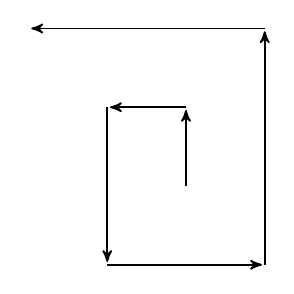
\begin{tikzpicture}[->,>=stealth',shorten >=1pt,auto,node distance=2.8cm,
                    semithick]
  \tikzstyle{every state}=[fill=red,draw=none,text=white]

  \coordinate  (A) at (0,0);
  \coordinate  (B) at (0,1);
  \coordinate  (C) at (-1,1);
  \coordinate  (D) at (-1,-1);
  \coordinate  (E) at (1,-1);
  \coordinate  (F) at (1,2);
  \coordinate  (G) at (-2,2);

  \path (A) edge (B)
        (B) edge (C)
        (C) edge (D)
        (D) edge (E)
        (E) edge (F)
        (F) edge (G);

\end{tikzpicture}
\caption{Bewegungsmuster Exploration -- circle}
\label{circle}
\end{figure}
\begin{figure}[h]
\centering
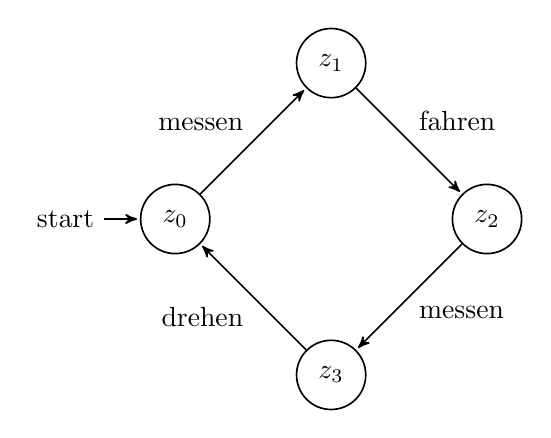
\begin{tikzpicture}[->,>=stealth',shorten >=1pt,auto,node distance=2.8cm,
                    semithick]
  \tikzstyle{every state}=[draw,text=black]

  \node[initial,state] (z0)                     {$z_0$};
  \node[state]         (z1) [above right of=z0] {$z_1$};
  \node[state]         (z2) [below right of=z1] {$z_2$};
  \node[state]         (z3) [below right of=z0] {$z_3$};


  \path (z0) edge node {messen} (z1)
        (z1) edge node {fahren} (z2)
        (z2) edge node {messen} (z3)
        (z3) edge node {drehen} (z0);

\end{tikzpicture}
\caption{state-machine Exploration -- circle}
\label{state_circle}
\end{figure}
\subsubsection{Exploration -- radar}
Wie in Abbildung \ref{radar} zu sehen ist, macht der Explorer eine Bewegungsabfolge in Form einer eckigen Wellenausbreitung. Durch diese Bewegungsfolge wird der Bereich vor dem Explorer schnell erkundet und der Explorer verlässt langsam seinen bisherigen Bereich.

Wie im Abschnitt Exploration -- circle wird hier auch ein Zustandsautomat (Abbildung \ref{state_radar}) zur Darstellung des Algorithmus verwendet. Er unterliegt den gleichen Kriterien wie oben.
\begin{figure}[h]
\centering
\begin{tikzpicture}[->,>=stealth',shorten >=1pt,auto,node distance=2.8cm,
                    semithick]
  \tikzstyle{every state}=[fill=red,draw=none,text=white]

  \coordinate  (A) at (0,0);
  \coordinate  (B) at (0,1);
  \coordinate  (C) at (2,1);
  \coordinate  (D) at (2,2);
  \coordinate  (E) at (-3,2);
  \coordinate  (F) at (-3,3);
  \coordinate  (G) at (5,3);

  \path (A) edge (B)
        (B) edge (C)
        (C) edge (D)
        (D) edge (E)
        (E) edge (F)
        (F) edge (G);

\end{tikzpicture}
\caption{Bewegungsmuster Exploration -- radar}
\label{radar}
\end{figure}
\begin{figure}[h]
\centering
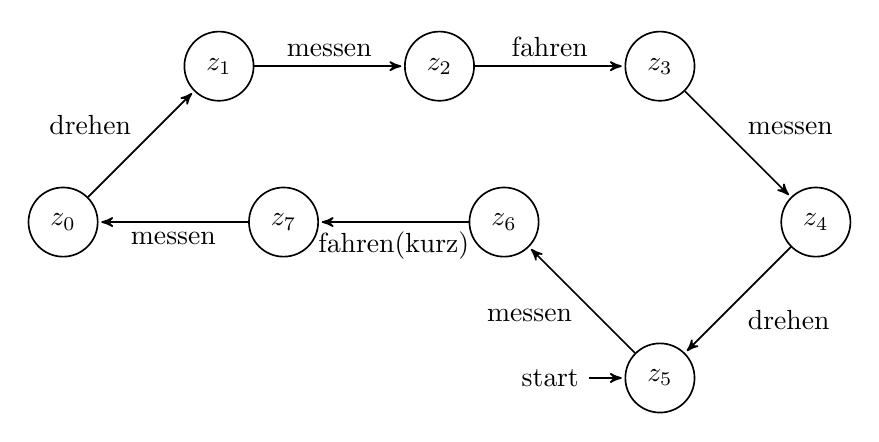
\begin{tikzpicture}[->,>=stealth',shorten >=1pt,auto,node distance=2.8cm,
                    semithick]
  \tikzstyle{every state}=[draw,text=black]

  \node[state]         (z0)                     {$z_0$};
  \node[state]         (z1) [above right of=z0] {$z_1$};
  \node[state]         (z2) [right of=z1] {$z_2$};
  \node[state]         (z3) [right of=z2] {$z_3$};
  \node[state]         (z4) [below right of=z3] {$z_4$};
  \node[initial,state]         (z5) [below left of=z4] {$z_5$};
  \node[state]         (z6) [above left of=z5] {$z_6$};
  \node[state]         (z7) [left of=z6] {$z_7$};


  \path (z0) edge node {drehen} (z1)
        (z1) edge node {messen} (z2)
        (z2) edge node {fahren} (z3)
        (z3) edge node {messen} (z4)
        (z4) edge node {drehen} (z5)
        (z5) edge node {messen} (z6)
        (z6) edge node {fahren(kurz)} (z7)
        (z7) edge node {messen} (z0);

\end{tikzpicture}
\caption{state-machine Exploration -- radar}
\label{state_radar}
\end{figure}
\subsection{GoToPoint}
Für die GoToPoint -- Funktionalität wurden die zwei Funktionen aus Listing \ref{listing1} und Listing \ref{listing2} benötigt. Mit der Funktion berechnePunkt() kann aus der eigenen Ausrichtung, der gefahrenen Entfernung und dem ehemaligen Standort der neu Standort berechnet werden. Die Funktion berechneVektor() aus Listing \ref{listing2} berechnet zu zwei gegebenen Punkten den verbindenden Vektor, dazu wird erst ein relatives Koordinatensystem geschaffen, dann wird über den Satz von Pythagoras die Entfernung, d.h. der Betrag des Vektor berechnet und danach Winkel berechnet.
\begin{figure}[h]
\begin{lstlisting}[language={python}, caption={berechnePunkt()}\label{listing1},captionpos=t]
def berechnePunkt(ausrichtung, entfernung, standort = {'x':0.0, 'y':0.0}):
    return {'x': standort['x'] + entfernung * GRAD2CM * 
                 math.cos(ausrichtung * (math.pi / 180.0)),
            'y': standort['y'] + entfernung * GRAD2CM * 
                 math.sin(ausrichtung * (math.pi / 180.0))}
\end{lstlisting}
\end{figure}
\begin{figure}[h]
\begin{lstlisting}[language={python}, caption={berechneVektor()}\label{listing2},captionpos=t]
def berechneVektor(standort = {'x':0.0, 'y':0.0}, ziel = {'x': 0.0, 'y': 0.0}):
    relativ_ziel = {'x': abs(ziel['x'] - standort['x']), 
                    'y': abs(ziel['y'] - standort['y'])}
    dbg_print("StO: (%d,%d), Z: (%d,%d), rZ: (%d,%d)"%(standort['x'],
                                                       standort['y'],
                                                       ziel['x'], 
                                                       ziel['y'], 
                                                       relativ_ziel['x'], 
                                                       relativ_ziel['y']), 1, 0)
    entfernung = math.sqrt(relativ_ziel['x'] ** 2 + relativ_ziel['y'] ** 2)
    if relativ_ziel['x'] == 0:
        winkel = 90
    elif relativ_ziel['x'] < 0:
        winkel = math.atan(float(relativ_ziel['y']) / float(relativ_ziel['x'])) * 
                 (180.0 / math.pi) + 180
    else:
        winkel = math.atan(float(relativ_ziel['y']) / float(relativ_ziel['x'])) * 
                 (180.0 / math.pi) + 360
    return {'winkel': winkel % 360, 
            'entfernung': entfernung, 
            'rel_x': relativ_ziel['x'], 
            'rel_y': relativ_ziel['y']}
\end{lstlisting}
\end{figure}

\chapter{NAO}\label{NAO}

\section{Vorüberlegungen}
Aus dem Szenario des Gesamtprojekts gingen bei unseren Vorüberlegungen zwei Hauptaufgaben für das NAO Team hervor. Zum einen ist das die Kalibrierung der NXT-Roboter während der Erkundungsphase auf unbekanntem Gebiet. Und zum anderen muss die Zielfindung des humanoiden NAO-Roboters, nachdem das Gebiet erkundet und eine konkrete Route zum Hotspot gefunden wurde, eingeleitet werden.
Unter der Kalibierung der NXT Roboters soll verstanden sein, dass der NAO Roboter mit Hilfe seiner Sensoren den NXT lokalisieren und diese berechnete Entfernung dem MCC mitteilen soll. Eine Kalibrierungsanfrage erfolgt immer nur aus Richtung des MCC an den NAO und zwar dann, wenn ein NXT ``verloren gegangen ist'', d.h. dieser keine genauen Daten mehr liefert.
Zunächst einmal bietet der Hersteller Aldebaran auf seiner Website%
	\footnote{http://www.aldebaran-robotics.com/documentation/index.html} eine recht umfangreiche Dokumentation. Diese ist, wie wir nach längerer Zeit aber feststellen mussten teilweise sehr schlecht. Es ist oft nicht klar, was die Daten, die man z.B. über die Sensoren abgreifen kann tatsächlich bedeuten. Dieses Problem trat beispielsweise bei den NAOMarks oder bei dem Sonar auf. In dem Abschnitt Probleme und Lösungen wird darauf noch eingegangen werden.
Gemeinsam mit den anderen Teams überlegten wir uns als einheitliche Programmiersprache Python zu verwenden, da sie sowohl von dem NXT-Mindstorm Robotern, als auch vom NAO unterstützt werden. Es hat sich allerdings herausgestellt das für die Programmiersprache C++ deutlich mehr Beispiele auf der Aldbaran Webseite vorliegen und die Dokumentation dafür besser ausgeführt ist.
Bei Aldebaran gibt es eine API, die es erlaubt vordefinierte Schnittstellen z.B. der Sensoren des NAOs zu benutzen.

\section{Software NAO}
\subsection{NAOqi}
NAOqi ist ein Framework von Aldebaran, was auf dem NAO läuft und den Roboter steuert. Es ist hardware- und plattformunabhängig. Für verschiedene Programmiersprachen wie z.B. C++ oder Python stellt Aldebaran ein Software Development Kit (SDK for NAOqi) bereit, um das Implementieren von Programmen auf dem NAO in verschiedenen Sprachen möglich zu machen.
Jede Maschine, auf der die NAOqi läuft, erschafft einen Broker. Jeder Broker verwaltet die Module, die innerhalb von ihm ausgeführt werden. Wenn ein Modul aufgebaut ist, bekommt es einen Zeiger auf den Broker übergeben. Module können Funktionen der anderen Module durch einen Proxy, der durch den Broker erzeugte wird, aufrufen.
Der Broker abstrahiert die Netzwerk-Schnittstelle auf den Maschinen, so dass, wenn eine Funktion über einen Proxy aufgerufen wird, diese Funktion möglicherweise auf einer anderen Maschine im Netzwerk ausgeführt werden kann.
\\
\begin{figure}[ht]
    \centering
	\includegraphics[width=0.7\textwidth, angle=0]{img/nao_1.png} 
\end{figure}
Innerhalb des NAOqi Prozesses laufen verschiedene Module. Wir verwenden diese Module:
\begin{enumerate}
\item ALLandMarkDetection: wird verwendet, um NAOMarks zu finden und zu erkennen
\item ALMemory: zum erignisbasierten Speichern von Daten
\item ALMotion: ansprechen der Motoren zum Bewegen des NAO
\item ALVideoDevice: erlaubt Zugriff auf die beiden Kameras des NAO
\end{enumerate}

\subsection{Choreographe}
Choreographe ist ein graphisches Programmierinterface. Durch das Auswählen und Verbinden von vorgefertigten Funktionsboxen kann man schnell und intuitiv erste Programme erzeugen und direkt auf dem NAO oder mit der Software NAOsim testen.
Alle Hauptfunktionen des NAOs wie beispielsweise die Steuerung aller Gelenke können mit verschiedensten Konfigurationen getestet werden. Dadurch ist dem Benutzer schnell ermöglicht erste Erfahrung mit dem Umgang des Roboters zu gesammelt. Wenn eine Verbindung zu einem NAO vorhanden ist, kann über ein dreidimensionales Robotermodell jeder Motor einzeln angesprochen werden. Darüber hinaus kann in einem weiteren Fenster das aktuelle Kamerabild angezeigt werden.
\subsection{Weitere Software}
\subsection*{NAOsim}
NAOsim ist ein Simulationsprogramm, womit ein vollständiger NAO simuliert werdern kann. Es ist möglich Testumgebungen selbst zu erschaffen, indem mach sich beispielsweise einen Raum mit Hindernissen einrichtet. Dadurch sind auch Tests einen realen NAO möglich. Auf einen realen Test sollte man allerdings keinesfalls verzichten, da NAOsim immer vollständig exakte Werte und Bewegungen des NAOs simuliert.
\subsection*{Monitor}
Dies ist ein Programm, dass das aktuelle Kamerabild oder alternativ die Sensordaten des NAOs auslesen und aufzeichnen kann. Das Programm ist vor allem dann hilfreich, wenn mit der Detektion von NAOMarkern gearbeitet wird. Es ist möglich über Monitor einzelne Einstellungen der Kamera wie beispielsweise Helligkeit, Kontrast, Gain, Auflösung, Sättigung oder Farbton vorzunehmen. 

\section{Hardware NAO}
In unseren Tests und für das Szenario selbst benutzen wir einen NAO H21 Body. Dieser zeichnet sich durch verschiedenste Sensoren aus. Es sind zwei Infrarotsensoren, drei Trägheitsmesser (2x Schwingungs- und 1x Beschleunigungssesoren), Kontaktsensoren für Brust, Füße und Kopf, Sonar (2 Empfänger und 2 Sender), 32 Positionssensoren, ein Force Sensing Resistor und vier Mikrofone, zwei Kameras, sowie zwei Lautsprecher eingebaut. Das vollständige Datenblatt kann man online bei Aldebaran anschauen%
	\footnote{http://www.technik-lpe.eu/fileadmin/bilder/produkte/aldebaran/NAO\_H21\_Next\_Gen.pdf}.

\section{Messungen}
Wie in dem Abschnitt Sensoren bereits beschrieben wurde, besitzt der NAO Roboter einige Sensoren, die wir vor der Benutzung auf die Genauigkeit verifiziert haben.
Wir haben Messreihen angelegt für die Vorwärtsbewegung des NAOs, also dem einfachen Laufen für das in dem Roboter integrierte Sonar und haben die Kamera auf Schärfe und Brauchbarkeit untersucht.

\subsection{Kamera}
Eine Herausforderung bei dem NAO stellt die integrierte Kamera dar. Da die Kommunikation drahtlos über ein WLan-Netzwerk sehr viel besser funktioniert, als mit Kabel, ist nur eine geringe Auflösung des Kamerabildes möglich (VGA). Alternativ kann auch eine höhere Auflösung (1280x960 Pixel) genutzt werden, dazu muss man aber gleichzeitig eine teilweise stark reduzierte Framerate (1 fps) in Kauf nehmen.
Zusammen mit der Kamera werden wichtige integrierte Funktionalitäten, wie die Erkennung von NAOMarkern und einem Roten Ball (mit genau definierter Größe), mitgeliefert. Diese werden in den nächsten Abschnitten genauer erklärt.

\subsection{Sonar}
Das Sonar des Roboters lässt sich relativ einfach über das bereits vorhandene Beispiel auf der Aldebaran Website%
	\footnote{http://www.aldebaran-robotics.com/documentation/\_downloads/sensors\_sonar.py} auslesen. Dabei gibt es zwei Sonarsensoren im NAO je einen für links und rechts. Die Ergebnisse können in dem hier vorliegenden Diagramm abgelesen werden. Wir habe für jeden Abstand zwischen 2.0 m und 0.1 m, die in 0.1 m Schritten weiter unterteilt sind, jeweils 10 Messungen entnommen und gemittelt. 
Es ist auffällig, aber nicht weiter verwunderlich, dass beim linken Sonar unseres NAOs die Genauigkeit abnimmt, je weiter er sich vom Hindernis entfernt. Beim rechten Sonar dagegen ist die Genauigkeit überraschenderweise auch bei einer Entferung von 1,5 m und größer weiterhin sehr gering (Abweichung < 1 cm). Sowohl bei dem linken, als auch dem rechten Sonar wird die Genauigkeit bei einer geringen Entfernung (<20 cm) gleichermaßen schlechter. 
Bei unseren Messungen haben wir keine Differenzierung in der Oberflächenbeschaffenheit unternommen, sodass unsere Messungen ausschließlich mit einer weißen glatten Wand als Hindernis durchgeführt wurden. Aussagen über andere Oberflächen können daher nicht gemacht werden.

\begin{figure}[ht]
    \centering
	\includegraphics[width=0.9\textwidth, angle=0]{img/nao_2.png} 
\end{figure}

\begin{figure}[ht]
    \centering
	\includegraphics[width=0.9\textwidth, angle=0]{img/nao_3.png} 
\end{figure}

\subsection{NAO Walk}
Für das Szenario unseres Semesterprojektes benötigen wir einen Roboter, der möglichst ohne Abweichungen laufen kann, um sein Ziel zu erreichen.
Man könnte auch annehmen, dass der NAO Roboter sich auf etwas größere Entfernungen trotzdem noch geradlinig bewegt. Dies ist tatsächlich aber nicht der Fall, da unser NAO schon bei kleineren Entfernungen einen deutlichen Drift nach rechts hatte. Um eine konkrete Aussage über die Genauigkeit des Laufens des NAOs treffen zu können und der Abweichung ggf. entgegenzuwirken, haben wir verschiedene Messreihen angelegt. Der NAO bietet über die bereits beschriebene mitgelieferte Software Choreographe die Möglichkeit verschiedenste Einstellungen der Laufbewegung einzustellen, was man natürlich auch über das NAOqi selbst implementieren kann. Einstellbare Parameter für den NAO Walk sind intuitiverweise die X- und Y-Bewegung, in der sich die Laufbewegung vorwärts (X positiv), rückwärts (X negativ), links (Y positiv) und rechts (Y negativ) wiederfinden lassen. Desweiteren gibt es den Parameter Theta, mit der man die Rotation des NAO definieren kann, wobei der Bereich [-1.0, 1.0] eingehalten werden muss und das Minimum (-1.0) die maximale Rotation im Uhrzeigersinn und das Maximum (1.0) die maximale Rotation gegen den Uhrzeigersinn widerspiegelt. Eine weiterere wichtige Einstellung, die man für das Laufen konfigurieren kann, ist die Schrittgröße sowohl für die X- (angegeben als ``MaxStepX''), als auch für die Y-Laufrichtung ``MaxStepY''). Dieser Wert liegt im Bereich von [0.1 cm; 6 cm].
Um zu erkennen welchen Einfluss die Schrittweite auf die Genauigkeit des Laufens an sich hat, haben wir jeweils 6 verschiedene Schrittweiten von 1 cm bis 6 cm in jeweils Zentimeterschritten genommen: Schrittweite\_i = 1 + i [cm] mit i = {0, 1, 2, 3, 4, 5}. Für jede Schrittweite wurden 5 Messungen vorgenommen und die Gesamtstrecke belief silch einmal auf 1 m und zum anderen auf 0.5 m, sodass insgesamt 60 Messungen vorgenommen wurden. Die Ergebnisse sind hier einmal in Tabellenform und einmal als Diagramm deutlich gemacht.
Zum Verständnis der Messergebnisse ist hier auch der Versuchsaufbau schematisch dargestellt.

\begin{figure}[ht]
    \centering
  \includegraphics[width=0.5\textwidth, angle=0]{img/nao_4.png}
    \caption{Der NAO läuft 0.5 bzw. 1 m; dx\_vorn und dx\_hinten sind die Abweichungen ausgehend von der Mittellinie zwischen den vorderen bzw. hinteren Füßen (ist der Wert positiv, dann gibt es ein Abdriften nach rechts, andernfalls links); dy gibt an, wie weit der NAO über das Ziel hinausgelaufen ist (ist der Wert positiv, dann ist er zu weit gelaufen, andernfalls zu wenig)}
    \label{nao_foot}
\end{figure}

\begin{figure}[ht]
    \centering
  \includegraphics[width=0.9\textwidth, angle=0]{img/nao_5.png}
    \caption{Abweichungen bei 0.5 m Entferung}
    \label{naotab3}
\end{figure}

\begin{figure}[ht]
    \centering
  \includegraphics[width=0.9\textwidth, angle=0]{img/nao_6.png}
    \caption{Abweichung bei 1 m Entfernung}
    \label{naotab4}
\end{figure}

\subsection{Auswertung}
Die Visualisierung des Diagramms macht bei beiden Entfernungen (0.5 m und 1 m) deutlich, dass je kleiner die Schrittweite des NAOs ist, die Abweichungen vom Ziel drastisch erhöhen. Daraus lässt sich schließen, dass beim Laufen eine möglichst hohe Schrittweite (Maximum von 6 cm) genommen werden sollte.
Außderdem wird deutlich, dass der NAO fast immer über sein Ziel hinausläuft (dy ist größer 0). 

\subsection{Fazit}
Die Messwerte für den NAO Walk sind scheinbar stark abhänig von Roboter selbst. Allerdings kann man sagen, dass die aufgezeigten Abweichungen insgesamt trotzdem relativ klassisch für NAO sind, da andere NAO Body auch immer ein Abdriften verzeichnet haben.
Um diese Abweichung beim Laufen zu verringern, könnte man die Messwerte mitteln und auf den Lauf anpassen. Allerdings kann man dadurch das Abdriften auch nicht verhindern, da man davon ausgehen muss das verschiedenste Faktoren, was bei uns nicht in die Messungen selbst mit eingeflossen ist, das Laufverhalten beeinflussen. So ist z.B. nicht komplett vorhersehbar, wie sich der Roboter auf einer völlig anderen Oberfläche als einem Teppich vortbewegt. Auch die Betriebsdauer des NAOs spielt hier eine entscheidende Rolle, da ein Roboter mit heißen oder sogar überhitzten Gelenken deutlich ungenauer in seiner Bewegung ist, als ein kurzzeitig eingeschalteter.
Auch wenn das Abdriften, wie bereits erwähnt, scheinbar klassisch für einen NAO ist, sollte man sich in einem Anwendungsszenario für Krisensituationen, wie wir es betrachten, sich nicht ausschließlich auf die Messungen stützen und den NAO kalibrieren. Diese Werte sind aber zu NAO-spezifisch und nicht allgemein genug, sodass hier klar geworden ist, dass man sich zur exakten Fortbewegung auf relative Bewegungen zurückgreifen sollte. D.h. der NAO soll sich möglichst selbstständig anhand seiner Umgebung neu orientieren und bei Abweichungen neu ausrichten. Dies könnte man bespielsweise durch Landmarken realisieren, was wir im nächsten Kapitel beschreiben werden.

\section{Kalibrierung}
Die Kalibrierung der NXT erfolgt mit Hilfe der NAO integrierten Kamera. Die Idee besteht darin, den NAO an eine feste Position am Rand des Feldes zu positionieren. Von diesem Punkt aus misst der NAO die Entfernung zum NXT, indem er diese mit seiner integrierten oberen Kamera erkennt und anschließend den Abstande berechnet.

\subsection{NAOMarker}
Um die NXTs überhaupt visuell zu erkennen werden sogenannte NAOMarker benutzt, die von dem NAO bereits standardmäßig erkannt werden. Auf der Aldebaran DVD gibt es genau 10 verschiedene NAOMarker, mit jeweils einer unterschiedlichen ID. Sollten diese Marker nicht ausreichen, werden online noch zusächliche angeboten, was wir allerdings nicht bestätigen können, da weder über den freien Zugang noch über den persönlichen Login weitere Marker zur Verfügung standen.

\begin{figure}[ht]
    \centering
  \includegraphics[width=0.3\textwidth, angle=0]{img/nao_7.png}
    \caption{Beispiel für einen NAOMarker mit ID 64.}
    \label{nao_marker}
\end{figure}

\subsection{Marker Konstruktion für NXT}
Da, wie bereits beschrieben, die NAOMarker mit der Erkennung von NXT-Robotern einher geht, haben wir uns Gedanken gemacht, wie ein oder mehrere Marker auf den “Erkundungsroboter” platziert werden können, um diese an möglichst jedem Punkt auf dem unbekannten Feld zu lokalisieren. Wir haben uns dafür entschieden sechs verschiedene Marker pro NXT zu verwenden, was von oben betrachtet einem gleichseitigen Hexagon entspricht. Auf den Bildern X und Y kann man diese noch einmal genauer sehen. Dadurch, dass wir von jeder Seite des NXTs eine andere ID erkennen, die einen NAOMarker codiert, können wir auf 60° genau die Drehung des NXTs unterscheiden. Dies wird unterteilt in 0° bzw. 360° (front), 60° (rechts vorn), 120° (rechts hinten), 180° (hinten), 240° (links hinten), 300° (links vorn). Daraus ergibt sich ein Vorteil: Bei unseren Tests haben wir festgestellt, dass sobald sich die Konstruktion in erkennbarer Reichweite für den NAO befindet, die Marker immer erkannt werden können, egal in welchem Winkel die Konstruktion zum NAO steht. D.h. ein Marker wird auch dann erkannt, wenn er im schlechtesten Fall in einem Winkel von 30° zur Kamera steht.

\begin{figure}[ht]
    \centering
  \includegraphics[width=0.9\textwidth, angle=0]{img/nao_8.png}
    \caption{Markerkonstruktion für NXT Roboter}
    \label{nao_marker2}
\end{figure}

Da wir unser Konstruktion auf einen relativ kleinen NXT platzieren und Einsparungen in der Größe der Marker machen wollten, haben wir den Kreis mit Struktur ausgeschnitten und auf den NXT platziert. Bei späteren Tests mit den ausgeschnittenen Markern haben wir allerdings herausgefunden, dass eine richtige Erkennung nur dann möglich ist, wenn er die auf dem Bild X die erkennbare Umrandung beibehält. Die Marker, die wir benutzen, sind wegen Platzgründen nur halb so Groß und im Durchmesser ca. 6 cm. Trotz kleinerer NAOMarker werden diese auch noch bei bis zu  160 cm erkannt. Man sollte außderdem wissen, dass die Erkennung der NAOMarker nur dann funktioniert, wenn die Marker wie in den Abbildungen im Hochformat vorliegt. Die Farbe ist allerdings egal nur die Struktur und der beschrieben Rand sind dagegen essentiell.
Da wir in unserem Szenario von drei NXTs ausgehen, die das Gelände erkunden und kalibriert werden müssen, bräuchten wir 18 Marker. Weil allerdings, wie bereits erwähnt, nur die 10 Marker vorhanden waren, haben wir uns dazu entschieden farbige Marker für die Unterscheidung zwischen den NXTs zu benutzen. Dies wird im Abschnitt X Farberkennung beschrieben.

\subsection{Auslesen der übergebenen Werte}
Die Markerinformationen können m.H. dieses Python Programmcodes abgegriffen werden: 
markerInfo = ALProxy(``ALMemory'', self.IP, self.PORT).getData``LandmarkDetected'')
\\
Die Daten in Form eines Arrays bei der Marker Detektion können wie folgt interpretiert werden: 
markerInfo = [[Zeitstempel\_in\_s, Zeitstempel\_in\_ms], [Markerarray\_0, Markerarray\_1, .. , Markerarray\_N], [MarkerInfoArray\_a], [MarkerInfoArray\_b]], Kamerainfo]
N ist die Anzahl der erkannten Marker. Je mehr der NAO an Marker erkennt, desto größer wird das Array mit den bereitgestellten Informationen. 
\\
Markerarray\_i, in der sich die spezifischen Daten für die Größe und Winkel der einzelnen Marker befindet, ist wie folgt aufgebaut:
Markerarray\_i = [[Form, Alpha, Beta, GroesseX, GroesseY, Titel], [MarkerID]].
MarkerInfoArray\_a und b sind jeweils sechs unbekannte Werte und auch bei Aldebaran nicht weiter kommentiert oder erklärt.
Was die Angaben für Form (shape) und Titel (heading) bedeuten, ist gänzlich unbekannt und die Dokumentation von Aldebaran gibt hier auch keine Informationen. Die Angabe zur Größe des erkannten Markers für X und Y sind zueinander immer gleich (abhängig von der Entfernung des Markers).
Die interessanten und für uns wichtigen Werte sind in Alpha und Beta gespeichert. Alpha gibt die Ausrichtung der Kamera nach rechts und links an, also den yaw-Winkel und Beta ist die Ausrichtung für oben und unten, also der pitch-Winkel. Alpha liegt in [-0.3, 0.3], wobei negative Werte rechts und positive Werte links vom Mittelpunkt des Kamerabildes liegen. Beta liegt  in [-0.25, 0.1], wobei negative Werte für oben und positive Werte für unten zu interpretieren sind.

\subsection{Farberkennung}
Da es von Aldebaran nur 10 frei verfügbare NAOMarker gibt, aber wir insgesamt 18 Marker brauchen, haben wir uns dafür entschieden jedem NXT die gleichen Marker mit unterschiedlichen Farben zuzuteilen. Dadurch ist es uns möglich über die Farbe den NXT zuzuordnen und über den Marker selbst die Ausrichtung des NXTs herauszufinden.
Die Triangulation ruft die Farberkennung auf, sobald ein Marker gefunden und auf ihn zentriert worden ist, der einem einem NXT zugeordnet werden soll. Die Farberkennung gibt dann die Farbe des zentrierten Markers zurück.
Zur Bildverarbeitung greifen wir auf OpenCV zu, das schon auf dem NAO installiert ist und viele vorgefertigte Methoden zum Verarbeiten bereitstellt.
\\
Zuerst nimmt die NAO Kamera ein Foto auf und speichert dies auf dem NAO. Zusätzlich wird der Pixelarray von dem Foto gespeichert, aus dem mit der Python Image Library ein Bild erzeugt wird. 
Danach wird anhand der gemessenen Markergröße ein Rechteck aus dem Bild ausgeschnitten, in dem sich der Marker befindet. Das Bild wird dann zu HSV(Hue, Saturation, Value) konvertiert, um leichter die Farbe bestimmen zu können.
Nun wird das Bild für jede Farbe nacheinander auf einen bestimmten HSV Bereich begrenzt bzw die Pixel in dem restlichen Bereich ausgeblendet. Um das Rauschen in den Fotos nicht zu berücksichtigen, wird ein Mindestbereich an Pixeln gewählt. Zusätzlich wird mit dem Pythagoras der Abstand des Bereichs zum Bildmittelpunkt berechnet. Im letzten Schritt werden die Bereiche von jeder Farbe miteinander verglichen und die Farbe mit dem Bereich, welche den kürzesten Abstand zum Mittelpunkt hat, als die wahrscheinlichste Farbe zurückgegeben. Falls keine der vorhandenen Farben gefunden wurde, dann wird dies zurückgegeben.


\subsection{Triangulation}
Die Idee zur Abstandsberechung durch Triangulation kam uns durch die Arbeit von [Stepan Krivanec et. al. 2009]\footnote{ftp://cmp.felk.cvut.cz/pub/cvl/articles/prusa/Krivanec-TR-2010-21.pdf}. In der Quelle wird beschrieben, dass eine Abstandsberechnung mit Hilfe der NAOMarker nur mit zwei NAOs möglich ist oder bei Bewegen des NAOs an eine andere Position, da der Roboter keine Stereo Kamera besitzen. Tatsächlich aber kann man auch über nur einen NAO triangulieren. Die Höhe der NAO-Kamera (obere Kamera) lässt sich einfach ausmessen und ist in der Initialpostition, wenn der NAO steht, genau 50 cm vom Boden entfernt. Außerdem werden, wenn ein NAOMarker erkannt wird, u.a. zwei Winkel zurückgegeben, die die horizontalen und vertikalen Winkel angeben, in dem sich die NAO Kamera zum Marker befindet.

\begin{figure}[ht]
    \centering
  \includegraphics[width=0.5\textwidth, angle=0]{img/nao_9.png}
    \caption{Darstellung des Aufbaus zur Markerdetektion}
    \label{nao_marker3}
\end{figure}

Mit Hilfe der Höhe und des Winkels kann nun Gleichung die Entfernungsberechnung erfolgen. Dazu verwenden wir die einfache trigonometrische Funktion   .
Die angepasste trigonometrische Funktion lautet:  . Der Winkel  kann aus dem bereits beschriebenen Markerarray\_i als Alpha extrahiert werden. 
Durch Umstellung erhalten wir den gesuchten Abstand mit  . Man beachte, dass in die Berechnung auch die Höhe des Markermittelpunktes Y eingeht und vorher genau ausgemessen werden sollte.

\section{NAOWalk mit RedBall Tracking}

Wie schon im Punkt ``4.3 NAOWalk'' beschrieben, ist der NAO nicht im Stande selbst kurze Strecken exakt zu laufen. Daher wäre es nicht möglich den NAO sich selbst über die Karte navigieren zu lassen. 
Um den NAO dennoch zum Ziel zu navigieren, ist es nötig Fixpunkte im Gelände zu haben, an denen er sich orientieren und seine Laufbahn korrigieren kann.
Realisiert werden diese Fixpunkte über einen roten Ball, den der NAO visuell erkennen und verarbeiten kann. Dieser ist auf einem der NXT's befestigt.
\\
Der Vorgang der Wegfindung basiert nun auf einem Pfad, den das MCC aus der Karte berechnet. Für diesen Vorgang verweise ich auf den Punkt Pfadberechnung in der MCC-Dokumentation.
Letztendlich entsteht dabei ein Pfad, der in Teilabschnitte unterteilt ist, die jeweils nur durch gerade Strecken miteinander verbunden sind.
\\
Entlang dieses Pfades wird der NXT mit dem roten Ball auf die bestimmten Positionen geschickt und der NAO folgt ihm.
Um zu verhindern dass der NAO und NXT sich gegenseitig in die Quere kommen werden die einzelnen Abschnitte des Pfades noch wie folgt in Phasen aufgeteilt, wobei die Ausgangsbedingung ist, dass sich der NXT eine Position weiter auf dem Pfad befindet als der NAO:
\\
P0: Sofern kein Nxt mit rotem Ball in Sicht ist, versuche einen zu finden
P1: NAO läuft gerade bis auf einige cm Abstand auf den NXT zu
P2: NAO speichert die Position des NXT
P3: NAO meldet dem MCC vor dem NXT angekommen zu sein
P4: MCC gibt NXT den Befehl, auf die nächste Position zu fahren
P5: NAO läuft auf die gespeicherte Position und richtet sich neu nach dem NXT aus
\\
Nach diesem Ablauf werden alle Teilabschnitte des Pfades abgearbeitet, bis der NAO sich im Zielgebiet befindet.
\\
Im Folgenden werden die einzelnen Fähigkeiten erklärt, die der NAO mitbringen muss, um oben genannte Phasen erfolgreich abschließen zu können.
\\
\\
\subsection*{P0:}
Der NAO muss entscheiden können, ob er einen roten Ball sieht oder nicht. Hierbei wird das NAOQi API Modul ALRedBallTracker benutzt, welche an das Event  redBallDetected() der ALRedBallDetection des ALVision-Moduls gekoppelt ist. ALRedBallTracker bietet die Funktion isNewData() an, welche true zurückgibt falls ein neuer roter Ball seit der letzten Abfrage erkannt worden ist. Um zu entscheiden, ob ein Ball erkannt wird, benutzt die Methode hasBall() der NAOWalk-Klasse diese Funktionalität.
\\
Liefert hasBall() false, so scannt er sein Blickfeld, indem er methodisch seinen Kopf derart bewegt, dass das maximal mögliche Sichtfeld abgedeckt wurde. Hat er danach noch immer nichts gefunden, dreht er sich um seine senkrechte Körperachse um 90 Grad und wiederholt den Vorgang bis er sich vollständig um die eigene Achse gedreht hat. Findet er letztendlich einen Ball, so richtet er sich nach diesem mit der privaten Methode \_\_turnToBall() aus. Diese Funktionalität bietet die retrieveBall()-Methode aus der NAOWalk-Klasse.
\\
\\
\subsection*{P1:}
Zusätzlich zu der Grundfunktionalität des Laufens in eine gegeben Richtung, welche über das ALMotion-Modul mittels der Methode walkTo()  gegeben wird, muss der NAO hierbei seine Laufbahn stetig korrigieren können. Da walkTo() dies per se nicht ermöglicht, muss eine Abweichung von der Laufbahn festgestellt werden können. Dies wird über eine Abfrage des Drehwinkels des Kopfgelenks realisiert. Die visuelle Erkennung des roten Balls ermöglicht es dem NAO, diesen permanent in der Mitte seines Sichtfeldes zu halten. Hierbei wird nur der Kopf bewegt. Bewegt sich der NAO relativ zum Ball, neigt bzw. dreht er den Kopf. Ab einer bestimmten Abweichung des Drehwinkels zum Nullpunkt ist davon auszugehen, dass der NAO seine gerade Bahn zum NXT verlassen hat und er wird gestoppt, richtet sich neu nach dem NXT mit turnToBall() aus und läuft erneut los.
\\
Da der Sichtbereich der oberen Kamera des NAO's bei aufgerichtetem Körper zu weit von ihm entfernt endet, um nah genug an den NXT heran zu kommen ohne ihn aus dem Blick zu verlieren, muss während der Annäherung ab einer bestimmten Distanz auf die untere Kamera umgeschaltet werden. Ein Beugen des Oberkörpers zu diesem Zweck führt zu einer erheblichen Instabilität der gesamten Laufanimation, sodass ein Hinfallen des Roboters unausweichlich ist. Dies geschieht über die beiden privaten Methoden \_\_setTopCamera() und \_\_setBottomCamera() der NAOWalk-Klasse.
\\
Zur Berechnung der Distanz wird die Methode getPosition() von ALRedBallTracker benutzt. 
Hierzu muss noch der SPACE\_TORSO eingeführt werden: 
NAO kennt verschiedene karthesische Räume, wie zum Bsp. SPACE\_TORSO, bei welchem ein 3D-Koordinatensystem in die Körpermitte des NAO gelegt wird. 
getPosition() liefert [x,y,z]-Koordinaten des Balls in SPACE\_TORSO zurück, wobei x die Distanz nach vorne bzw hinten, y nach rechts bzw links und z die Höhe ist. 
\\
Um festzustellen, ob die Rückgabewerte von getPosition() für eine automatisierte  Verarbeitung geeignet sind, wurde eine Testreihe angelegt, deren Ergebnis dem Diagramm unten zu entnehmen ist. Real bezeichne dabei die in der realen Welt gemessenen Werte.

\begin{figure}[ht]
    \centering
  \includegraphics[width=0.9\textwidth, angle=0]{img/nao_10.png}
\end{figure}

Es ist deutlich zu sehen, dass der Werteverlauf bei x sowie y linear ist. z kann hierbei ignoriert werden, da es für die Berechnung des Abstandes irrelevant ist. Die geringen Abweichungen  ergeben sich aus Messungenauigkeiten. 
Daraus folgt, dass die cm in SPACE\_TORSO sich aus den Rückgabewerten mittels einer linearen Funktion in cm in real interpolieren lassen. 
Ergo ipso facto lassen sich exakte Werte zur Weiterverarbeitung gewinnen.
\\
Da die Höhe des Balls konstant bleibt, lässt sich der Abstand aus der Auslenkung der x- und y-Achse interpolieren. Dies geschieht mit einem simplen Pythagoras und ist in die private Methode \_\_getDistance() ausgelagert.
Diese gesamte Funktionalität ist in der walkUpToBall()-Methode aus der NAOWalk-Klasse implementiert.
\\
\\
\subsection*{P2:}
Um die Position eines NXT zu speichern legt der NAO ein Datenfeld mit den Koordinaten der getPosition()-Methode zum Zeitpunkt der Speicherung mittels \_\_safePosition() an. Nun kann er diese Daten benutzen, wenn sich der NXT schon auf die nächste Position bewegt hat.
\\
\\
\subsection*{P5:}
Aus der vorher gespeicherten Position relativ zum NAO in SPACE\_TORSO, kann der NAO nun interpolieren, wie weit er sich bewegen muss um exakt auf dieser Position zu stehen. Dies geschieht in der walkToPosition()-Methode der NAOWalk-Klasse. Dieser Abstand ist sehr kurz und kann daher ohne korrektur vom NAO gelaufen werden.
Sollte sich der NAO noch nicht im Zielgebiet befinden, richtet er sich mit retrieveBall() erneut nach dem NXT mit dem roten Ball aus und der Phasendurchlauf beginnt von vorne.

\section{Probleme \& Lösungen}

\subsection{NAO}
Am Anfang haben wir uns immer direkt mit einem LAN Kabel zu dem NAO verbunden, wobei diese Verbindung sehr störanfällig war. 
Die Konnektivität erfolgte später über WLAN. Dies war sehr viel stabiler und störunanfälliger, jedoch kam es häufig trotzdem zu Verbindungsproblemen, die meistens mit einem Neustart des NAO behoben werden konnten.
Die Sensoren des NAO waren bei uns teilweise sehr anfällig und ungenau.
Wenn der NAO längere Zeit mit Stiffness stand, dann haben sich die Motoren so stark erhitzt, dass der NAO erst abkühlen musste bevor er weiter verwendet werden konnte.
Teilweise ist auch das NAOqi grundlos abgestürzt und der NAO ist daraufhin einfach hingefallen.

\subsection{NAOMarker}
Der NAO sollte eigentlich maximal 6 Marker gleichzeitig erkennen, jedoch hat er bei uns auch mehr Marker gleichzeitig erkannt. Die Markererkennung arbeit auf einem bestimmten Bereich vor dem NAO, ca. zwischen 20 cm und 140 cm, akkurat. Wenn der Marker jedoch näher oder weiter entfernt ist, dann erkennt der NAO den Marker entweder überhaupt nicht oder verwechselt ihn mit einem anderen Marker.

\subsection{Triangulation}
Die Triangulation schwankt durch die Ungenauigkeit der Markererkennung, wodurch die Abweichung bis zu 10 cm betragen kann.

\subsection{Farberkennung}
Die Bilder der Kamera sind durch die verschiedenen Beleuchtungsverhältnisse sehr unterschiedlich von der Helligkeit und dem Kontrast. Am Anfang haben wir Versuche mit der Farbe gelb und später schwarz durchgeführt, jedoch war gelb immer zu schwer von weiß und schwarz zu schwer vom Untergrund zu unterscheiden und deshalb sind diese weggefallen. Bei den anderen Farben haben wir es nach vielen Feinjustierungen geschafft, die unterschiedlichen Farben über verschiedene Distanzen zu erkennen.
Durch die Zentrierung der Kamera NAO auf die einzelnen Marker wurde auch das Problem der verschiedenen Farbbereiche im Sichtfeld, wobei nicht nach der Größe der Farbbereiche beurteilt werden darf, gelöst.
Die Farberkennung dauerte am Anfang auch sehr lange, aber konnte durch die Wahl des Bildtyps von JPG anstatt PNG stark beschleunigt werden.\\
\part{Fazit}
\startcontents[parts]
\rtHrule
\vskip 20pt
\printcontents[parts]{}{0}{\setcounter{tocdepth}{2}}
\vskip 20pt
\rtHrule
\chapter{Fazit}\label{Fazit}

\section{Aufgabenstellung}
Die gegebene Aufgabenstellung umfasst viele Teilgebiete des Bachelor-Studiengangs Informatik an der Humboldt-Universität. Es werden sowohl gute Kenntnisse im Bereich Software-Engineering, Kommunikationssysteme und ein gutes Gefühl für Algorithmen benötigt als auch ein grundlegendes Wissen im Bereich mathematischer Problemstellungen, dass über die vermittelten Inhalte des Abiturs hinausgeht. Außerdem bietet sich die Möglichkeit einen Einblick in die Arbeit mit verschiedenen Robotern zu bekommen - wobei sich dieser Aspekt, auf Grund des kleinen Zeitfensters, nur auf sehr rudimentäre Anwendungen beschränkt.
Die Problemstellung ermöglicht eine gute und sinnvolle Unterteilung in Kleingruppen, die unter Einhaltung vereinbarter Schnittstellen unabhängig voneinander arbeiten können. Diese Teilaufgaben bieten weiterhin  die Möglichkeit, sich für ein gewisses Themengebiet zu entscheiden: Für die NXT's ist eine gewisse Kreativität und handwerkliches Geschick erforderlich, da die Modelle, bzw. das endgültige Modell, viele Anforderungen an seine Umgebung und seine Funktionalität erfüllen muss; Der NAO-Roboter bietet die Möglichkeit der Bilderkennung; die MCC-Gruppe hat hauptsächlich algorithmische Probleme zu lösen.
Wie bereits in der Aufgabenstellung zitiert, ist das Problem sehr Anwendungsorientiert - auch wenn es keinen direkten Forschungsbezug gibt, so gewinnt man doch einen sehr guten Eindruck davon, wie zukünftig Roboter bei realen Problemen aushelfen können und vor welchen Schwierigkeiten die Entwickler und Ingenieure stehen.

\section{Projektplanung}
Die größte Hürde der meisten Projekte ist die Projektplanung. Nicht nur ein Vorgehensmodell für die Softwareentwicklung, sowie eine exakte Erfassung von Anforderung sind hier notwendig, sondern auch eine gute Planung auf Ebene der gesamten Gruppe. Das heißt, eine unabhängige Kleingruppenarbeit ist nur möglich wenn die Schnittstellen einvernehmlich und präzise definiert wurden. Ein Integrations- und Systemtest ist nur möglich wenn alle Teilaufgaben bis zu einem vereinbarten Zeitpunkt fertig sind. Ein erfolgreicher Abschluss ist nur möglich wenn von Anfang ein genauer Projektplan ausgearbeitet wird, der es ermöglicht, bei nicht haltbaren Fristen entsprechend zu reagieren.
Auch in diesem Projekt hat sich die fehlende Erfahrung deutlich bemerkbar gemacht, insbesondere dadurch, dass letztendlich kein vollständig autonomer Ablauf bei der Abschlusspräsentation möglich war. Es ist offensichtlich, dass nicht nur Wissen in den oben genannten Fachgebieten von Nöten ist, sondern auch eine zumindest grundsätzliche Einführung in Projektmanagement wichtig wäre.
Die Projektplanung umfasst häufig auch den Einsatz bestimmter Werkzeuge während des Projekts. Hier bestand das Problem, dass es, abgesehen vom Versionierungstool ``GIT'', keine einheitliche Verwendung von Tools zur Dokumentation, Verteilung von Aufgaben, Software-Entwicklung und Software-Entwurf gab. 
Auch die Verwendung der verschiedenen Plattformen (MAC, Windows, Linux) bereitete insbesondere im Bereich der Visualisierung erhebliche Probleme.
Zuletzt scheint auch Entscheidung für Python als durchgängig zu verwende Programmiersprache keine gute gewesen zu sein. Allerdings muss an dieser Stelle gesagt werden, dass die damit verbunden Probleme keineswegs vorhersehbar gewesen sind.
\\
Abschließend lässt sich sagen, dass doch ein sehr erheblicher Teil der Arbeitszeit und des letztendlichen Projektergebnisses der ungenügenden Projektplanung zuzuschreiben sind - es wäre sicherlich sehr zielführend, wenn die Studierenden in zukünftigen Projekten explizit auf diese Herausforderung vorbereitet werden.

\section{Aussicht}
Aus unserer Sicht war das Semesterprojekt trotz der genannten Probleme nicht nur sehr lehrreich, sondern die meiste Zeit auch eine Bereicherung für die Teilnehmer. Insbesondere kann man aus den größeren aufgetretenen Problemen viel lernen, um es in zukünftigen Projekten besser zu machen.
Das Themengebiet bietet im allgemeinen unzählige Möglichkeiten an weiteren Projekten teilzunehmen, Abschlussarbeiten zu schreiben oder Forschung zu betreiben. Durch das Semesterprojekt hat man einen weit gefächerten Einblick in die Thematik erhalten. Die Aufgabe hat gezeigt, wie weit der Schritt zu einem tatsächlich autonom agierenden Roboterteam in einem unwegsamen Gelände noch ist.
\end{document}
